%%%%%%%%%%%%%%%%%%%%%%%%%%%%%%%%%%%%%%%%%
% Wenneker Article
% LaTeX Template
% Version 2.0 (28/2/17)
%
% This template was downloaded from:
% http://www.LaTeXTemplates.com
%
% Authors:
% Vel (vel@LaTeXTemplates.com)
% Frits Wenneker
%
% License:
% CC BY-NC-SA 3.0 (http://creativecommons.org/licenses/by-nc-sa/3.0/)
%
%%%%%%%%%%%%%%%%%%%%%%%%%%%%%%%%%%%%%%%%%

%----------------------------------------------------------------------------------------
%	PACKAGES AND OTHER DOCUMENT CONFIGURATIONS
%----------------------------------------------------------------------------------------
\documentclass[10pt, a4paper, twocolumn]{article} % 10pt font size (11 and 12 also possible), A4 paper (letterpaper for US letter) and two column layout (remove for one column)

%%%%%%%%%%%%%%%%%%%%%%%%%%%%%%%%%%%%%%%%%
% Wenneker Article
% Structure Specification File
% Version 1.0 (28/2/17)
%
% This file originates from:
% http://www.LaTeXTemplates.com
%
% Authors:
% Frits Wenneker
% Vel (vel@LaTeXTemplates.com)
%
% License:
% CC BY-NC-SA 3.0 (http://creativecommons.org/licenses/by-nc-sa/3.0/)
%
%%%%%%%%%%%%%%%%%%%%%%%%%%%%%%%%%%%%%%%%%

%----------------------------------------------------------------------------------------
%	PACKAGES AND OTHER DOCUMENT CONFIGURATIONS
%----------------------------------------------------------------------------------------
\usepackage{hyperref}
\hypersetup{
    colorlinks=true,
    linkcolor=blue,
    filecolor=magenta,      
    urlcolor=cyan,
}
 
\urlstyle{same}

\usepackage{wrapfig}

\usepackage[english]{babel} % English language hyphenation

\usepackage{microtype} % Better typography

\usepackage{amsmath,amsfonts,amsthm} % Math packages for equations

\usepackage[svgnames]{xcolor} % Enabling colors by their 'svgnames'

\usepackage[hang, small, labelfont=bf, up, textfont=it]{caption} % Custom captions under/above tables and figures

\usepackage{booktabs} % Horizontal rules in tables

\usepackage{lastpage} % Used to determine the number of pages in the document (for "Page X of Total")

\usepackage{graphicx} % Required for adding images
\usepackage[export]{adjustbox}

\usepackage{enumitem} % Required for customising lists
\setlist{noitemsep} % Remove spacing between bullet/numbered list elements

\usepackage{sectsty} % Enables custom section titles
\allsectionsfont{\usefont{OT1}{phv}{b}{n}} % Change the font of all section commands (Helvetica)

%----------------------------------------------------------------------------------------
%	MARGINS AND SPACING
%----------------------------------------------------------------------------------------

\usepackage{geometry} % Required for adjusting page dimensions

\geometry{
	top=1cm, % Top margin
	bottom=1.5cm, % Bottom margin
	left=2cm, % Left margin
	right=2cm, % Right margin
	includehead, % Include space for a header
	includefoot, % Include space for a footer
	%showframe, % Uncomment to show how the type block is set on the page
}

\setlength{\columnsep}{7mm} % Column separation width

%----------------------------------------------------------------------------------------
%	FONTS
%----------------------------------------------------------------------------------------

\usepackage[T1]{fontenc} % Output font encoding for international characters
\usepackage[utf8]{inputenc} % Required for inputting international characters

\usepackage{XCharter} % Use the XCharter font

%----------------------------------------------------------------------------------------
%	HEADERS AND FOOTERS
%----------------------------------------------------------------------------------------

\usepackage{fancyhdr} % Needed to define custom headers/footers
\pagestyle{fancy} % Enables the custom headers/footers

\renewcommand{\headrulewidth}{0.0pt} % No header rule
\renewcommand{\footrulewidth}{0.4pt} % Thin footer rule

\renewcommand{\sectionmark}[1]{\markboth{#1}{}} % Removes the section number from the header when \leftmark is used

%\nouppercase\leftmark % Add this to one of the lines below if you want a section title in the header/footer

% Headers
\lhead{} % Left header
\chead{\textit{\thetitle}} % Center header - currently printing the article title
\rhead{} % Right header

% Footers
\lfoot{} % Left footer
\cfoot{} % Center footer
%\rfoot{\footnotesize Page \thepage\ of \pageref{LastPage}} % Right footer, "Page 1 of 2"

\fancypagestyle{firstpage}{ % Page style for the first page with the title
	\fancyhf{}
	\renewcommand{\footrulewidth}{0pt} % Suppress footer rule
}

%----------------------------------------------------------------------------------------
%	TITLE SECTION
%----------------------------------------------------------------------------------------

\newcommand{\authorstyle}[1]{{\large\usefont{OT1}{phv}{b}{n}\color{DarkRed}#1}} % Authors style (Helvetica)

\newcommand{\institution}[1]{{\footnotesize\usefont{OT1}{phv}{m}{sl}\color{Black}#1}} % Institutions style (Helvetica)

\usepackage{titling} % Allows custom title configuration

\newcommand{\HorRule}{\color{DarkGoldenrod}\rule{\linewidth}{1pt}} % Defines the gold horizontal rule around the title

\pretitle{
	\vspace{-30pt} % Move the entire title section up
	\HorRule\vspace{10pt} % Horizontal rule before the title
	\fontsize{32}{36}\usefont{OT1}{phv}{b}{n}\selectfont % Helvetica
	\color{DarkRed} % Text colour for the title and author(s)
}

\posttitle{\par\vskip 15pt} % Whitespace under the title

\preauthor{} % Anything that will appear before \author is printed

\postauthor{ % Anything that will appear after \author is printed
	\vspace{10pt} % Space before the rule
	\par\HorRule % Horizontal rule after the title
	\vspace{20pt} % Space after the title section
}

%----------------------------------------------------------------------------------------
%	ABSTRACT
%----------------------------------------------------------------------------------------

\usepackage{lettrine} % Package to accentuate the first letter of the text (lettrine)
\usepackage{fix-cm}	% Fixes the height of the lettrine

\newcommand{\initial}[1]{ % Defines the command and style for the lettrine
	\lettrine[lines=3,findent=4pt,nindent=0pt]{% Lettrine takes up 3 lines, the text to the right of it is indented 4pt and further indenting of lines 2+ is stopped
		\color{DarkGoldenrod}% Lettrine colour
		{#1}% The letter
	}{}%
}

\usepackage{xstring} % Required for string manipulation

\newcommand{\lettrineabstract}[1]{
	\StrLeft{#1}{1}[\firstletter] % Capture the first letter of the abstract for the lettrine
	\initial{\firstletter}\textbf{\StrGobbleLeft{#1}{1}} % Print the abstract with the first letter as a lettrine and the rest in bold
}

%----------------------------------------------------------------------------------------
%	BIBLIOGRAPHY
%----------------------------------------------------------------------------------------

\usepackage[backend=bibtex,style=authoryear,natbib=true]{biblatex} % Use the bibtex backend with the authoryear citation style (which resembles APA)

\addbibresource{example.bib} % The filename of the bibliography

\usepackage[autostyle=true]{csquotes} % Required to generate language-dependent quotes in the bibliography
 % Specifies the document structure and loads requires packages

%----------------------------------------------------------------------------------------
%	ARTICLE INFORMATION
%----------------------------------------------------------------------------------------

\title{Titanic Data Analysis Report} % The article title

\author{
	\authorstyle{Chen Qingqing\textsuperscript{1}} % Authors
	\newline\newline % Space before institutions
	\textsuperscript{1}\institution{Udacity Data Analyst Nanodegree Program Student, Singapore}\\ % Institution 1
	%\textsuperscript{2}\institution{University of Texas at Austin, Texas, United States of America}\\ % Institution 2
	%\textsuperscript{3}\institution{\texttt{LaTeXTemplates.com}} % Institution 3
}

% Example of a one line author/institution relationship
%\author{\newauthor{John Marston} \newinstitution{Universidad Nacional Autónoma de México, Mexico City, Mexico}}

\date{Feb 20, 2018} % Add a date here if you would like one to appear underneath the title block, use \today for the current date, leave empty for no date

%----------------------------------------------------------------------------------------

\begin{document}

\maketitle % Print the title

%\thispagestyle{firstpage} % Apply the page style for the first page (no headers and footers)

%----------------------------------------------------------------------------------------
%	ABSTRACT
%----------------------------------------------------------------------------------------

\lettrineabstract{The sinking of the RMS Titanic is one of the most infamous shipwrecks in history.  On April 15, 1912, during her maiden voyage, the Titanic sank after colliding with an iceberg, killing 1502 out of 2224 passengers and crew. This sensational tragedy shocked the international community and led to better safety regulations for ships. One of the reasons that the shipwreck led to such loss of life was that there were not enough lifeboats for the passengers and crew. Although there was some element of luck involved in surviving the sinking, some groups of people were more likely to survive than others, such as women, children, and the upper-class. In this project, I am going to create a visualization that shows the demographics or passenger information between those passengers who survived and those who died.}

%----------------------------------------------------------------------------------------
%	ARTICLE CONTENTS
%----------------------------------------------------------------------------------------

\section{Choose a Data Set}

A data set is choose from the \href{https://docs.google.com/document/d/1w7KhqotVi5eoKE3I_AZHbsxdr-NmcWsLTIiZrpxWx4w/pub?embedded=true}{Data Set Options} document (\textbf{Titanic Data}). In this dataset, it contains demographics and passenger information from a subset of the 2224 passengers and crew on board the Titanic. 

%------------------------------------------------
\section{Exploratory of Data Analysis}


%------------------------------------------------

\subsection{Data description}

The variables on the dataset are Passenger ID, Survived, Pclass, Name, Sex, Age, SibSp, Parch, Ticket, Fare, Cabin and Embarked. 

\begin{enumerate}
	\item Pclass: Passenger Class (1 = 1st (Upper); 2 = 2nd (Middle); 3 = 3rd (Lower))
	\item Survived: 0 = No; 1 = Yes
	\item Age: age is in Years; Fractional if Age less than One (1); If the Age is estimated, it is in the form xx.5
	\item SibSp: Number of Siblings/Spouses Aboard 
	\item Parch: Number of Parents/Children Aboard
	\item Fare: Passenger Fare (British pound), is in Pre-1970 British Pounds;  Conversion Factors: 1 = 12s = 240d and 1s = 20d
	\item Embarked: Port of Embarkation (C = Cherbourg; Q = Queenstown; S = Southampton)
\end{enumerate}


%------------------------------------------------
\subsection{Data Wrangling}

After visually looking at the dataset, I started data wrangling. First, I checked whether there was any null or duplicated passenger IDs, and dropped them.  Then I modified columns of the dataset with the following steps and finally saved the modified dataset to a new csv file named \textbf{"clean.csv"}.
\begin{enumerate}
	\item Pclass column: Replace number "1, 2, 3" with "Upper, Middle, Lower" separately; 
	\item Survived column: Replace number "0 and 1" with "Not survived, survived";  
	\item Age column: Divide age to different ranges (0-10, 11-20, 21-30, 31-40, 41-50, 51-60, 61-70, 71-80)
	\item Embarked column: Replace capital characters "C, Q, S" to "Cherbourg, Queenstown, Southampton" separately;
\end{enumerate}
%------------------------------------------------

\section{Create Visualization}
In this section, a visualizaition was created using \textbf{Tableau} to explain and help lead a reader to identify some key insights into the dataset.  And there were two versions of the visualizaiton. One was initial version which could be found through this link: \href{https://public.tableau.com/profile/qingqing2461#!/vizhome/TitanicDataAnalysisReport_first_version/1_title}{\textbf{First Version}}, and another one was the final version which had some modifications after getting the feedback from readers and it could be found through this link: \href{https://public.tableau.com/profile/qingqing2461#!/vizhome/TitanicDataAnalysisReport/Data_report?publish=yes}{\textbf{Final Version}}.

Firstly, I put passengers basic information in my story line and added filters like "Survival status, sex, ticket number, and embarked place. This was in order to help reader to find the passenger easier. Then I used bar plot to show detailed difference between survived and not survived passengers in sex. classes, and embarked place. For total 340 survived passengers, 67.94\% is female and 32.06\% is male; and for total 549 died passengers, 85.25\% is male and 14.75\% is female. The survived passengers percentage of upper class is higher than middle and lower class passengers. Mostly, the passengers were embarked at Southampton.[Figure1]

\begin{figure}
	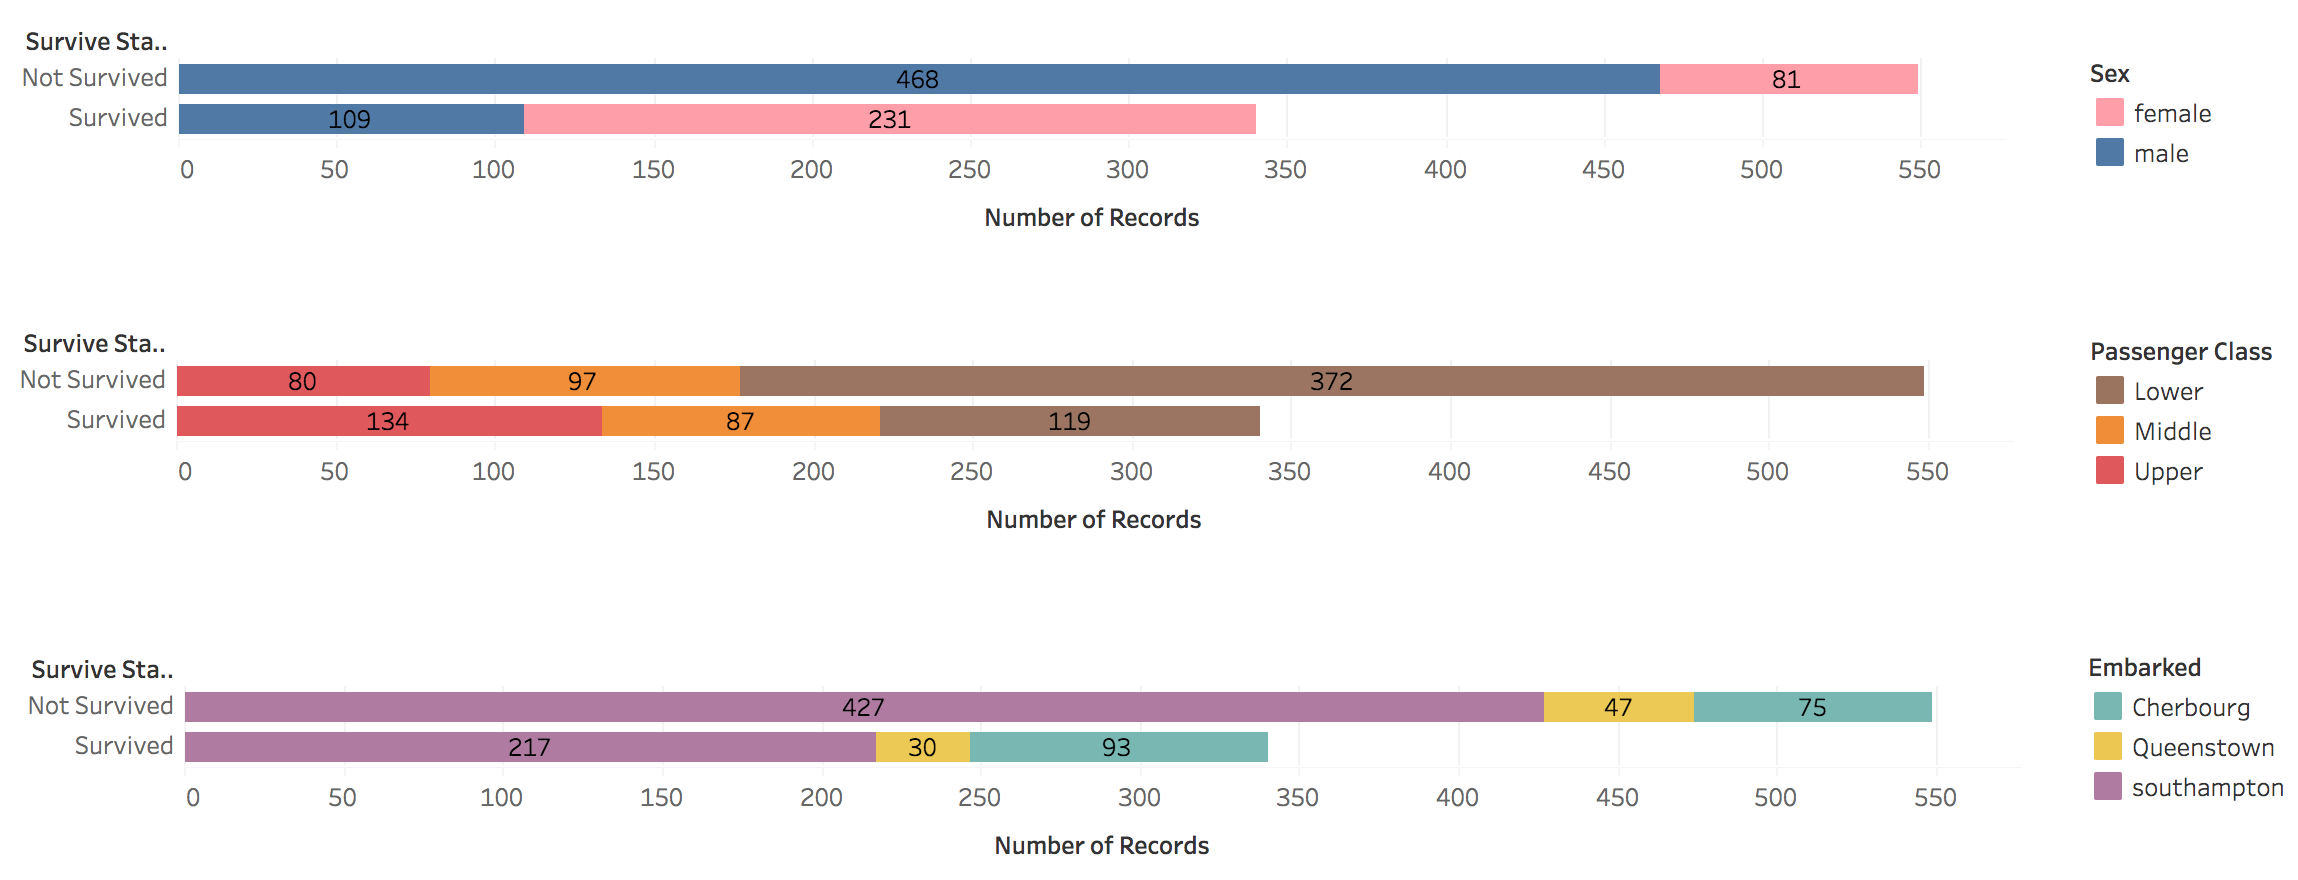
\includegraphics[width=\linewidth]{1-1.png} % Figure image
	%\caption{Sex, class level and embarked place information for survived and not survived passengers} % Figure caption
	%\label{bear} % Label for referencing with \ref{bear}
\end{figure}

\begin{figure}
	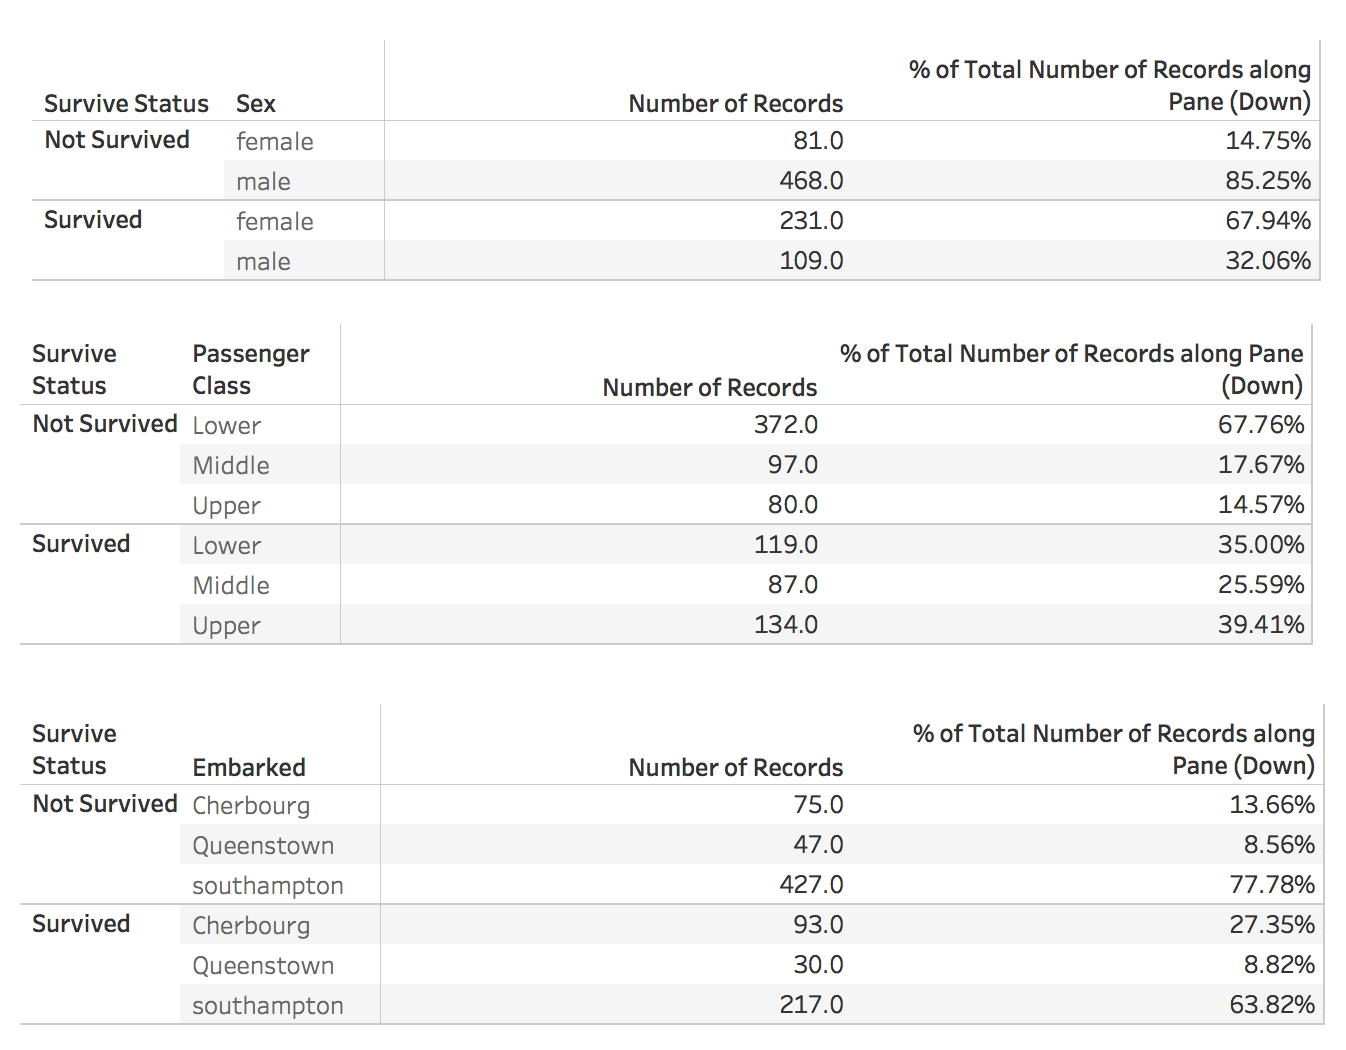
\includegraphics[width=\linewidth]{1.png} % Figure image
	\caption{Sex, class level and embarked place information for survived and not survived passengers} % Figure caption
	%\label{bear} % Label for referencing with \ref{bear}
\end{figure}

\begin{figure}[h]
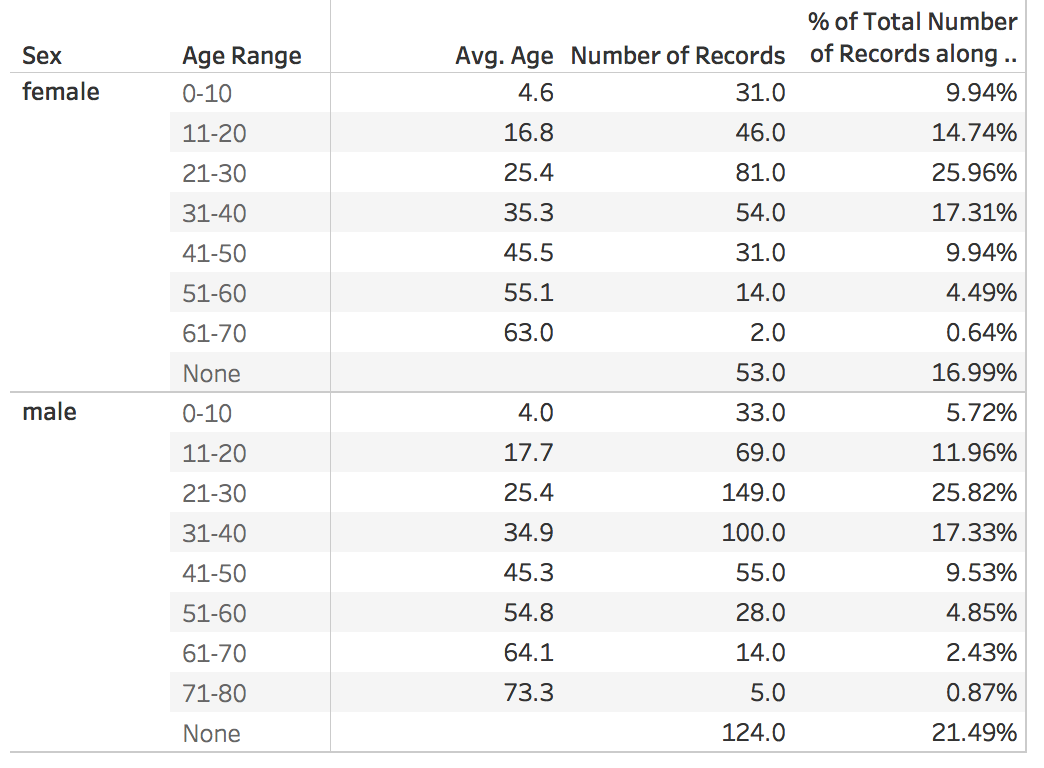
\includegraphics[width=\linewidth, height=5cm, right]{2.png} % Figure image
\caption{Age range information for survived and not survived passengers} % Figure caption
\label{bear} % Label for referencing with \ref{bear}
\end{figure}

For female, mostly the age is between 11 - 40 years old, the age in range of 21 to 30 years old has the highest percentage which is 25.96\%; the age under 10 years old and above 60 years old is relatively less than other age ranges. 
For male, mostly the age is between 11-40 years old, the age in range of 21 to 30 years old has the highest percentage which is 25.82\%;  the age under 10 years old and above 60 years old is relatively less than other age ranges. [figure 2]

	
Then I used box plot and histogram to show the average fare between different genders and among different class levels. Because it is easier and more obvious for readers to see the highest, median and lowest average fares and it is clear for readers to compare the fares in different classes. The average fare of female in different class is higher than that of male, and the average fare for upper class passengers is higher than other two classes passengers in both male and female.

Mostly passengers bring the children together with them where there is 22.10\% and 32.08\% passengers is under 10 years old for not survived and survived passengers.

There are 27.3\% and 21.60\% siblings is under 10 years old for not survived and survived passengers.
\begin{figure}[h]
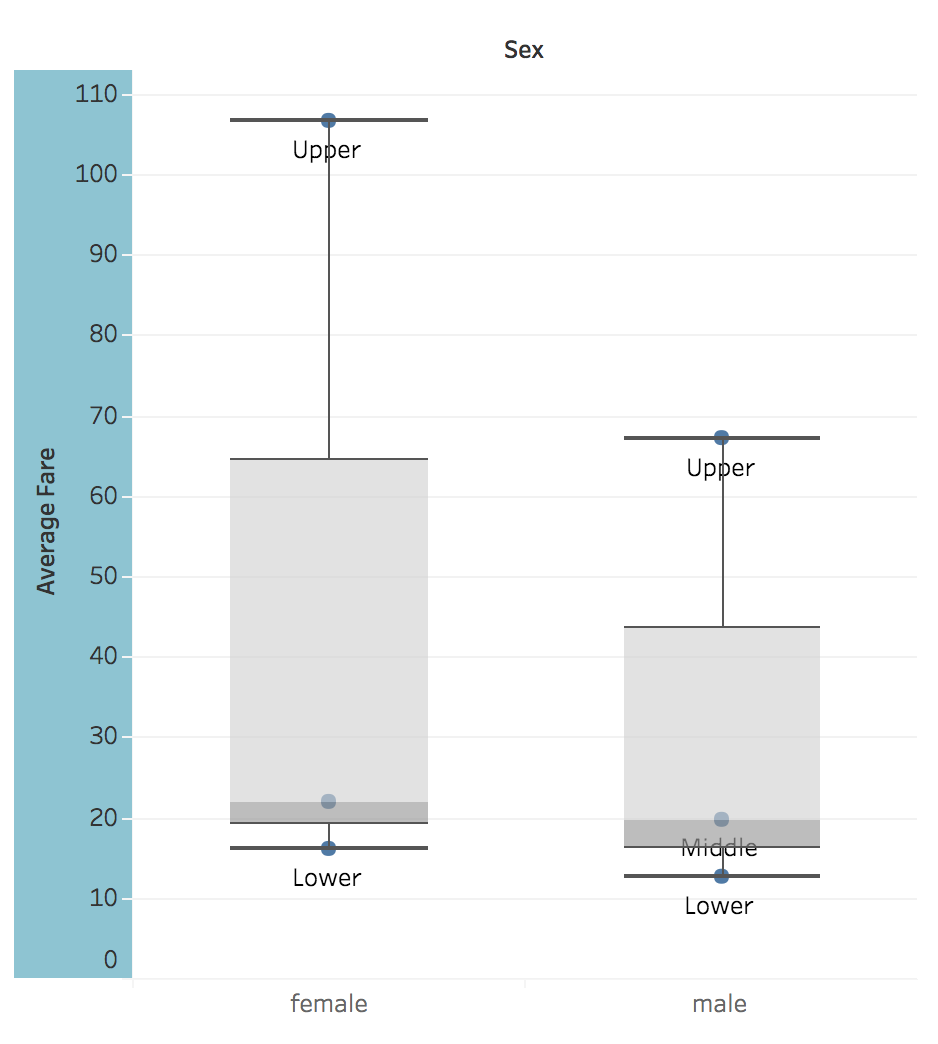
\includegraphics[width=\linewidth]{3-1.png} % Figure image
%\caption{Age range information for survived and not survived passengers} % Figure caption
%\label{bear} % Label for referencing with \ref{bear}
\end{figure}



%----------------------------------------------------------------------------------------
\section{Get Feedback and Improve the Visualization }
\subsection{Get Feedback }
\begin{enumerate}
	\item Advantage: There is a clear story line shown in the Tableau that I can understand all of the contents in the slides and all the calculation and plots are correct;
         \item Disadvantage: It would be better if there will be some comments or conclusion for each slide;  
	\end{enumerate}
\subsection{Improve the Visualization}


Based on the feedback, I add the conclusion in the slides to make it more understandable and I also add one picture in the title slide in order to catch readers' eyes.

%----------------------------------------------------------------------------------------
%	BIBLIOGRAPHY
%----------------------------------------------------------------------------------------

%\printbibliography[title={Bibliography}] % Print the bibliography, section title in curly brackets

%----------------------------------------------------------------------------------------

\end{document}
